% Template for ICIP-2019 paper; to be used with:
%          spconf.sty  - ICASSP/ICIP LaTeX style file, and
%          IEEEbib.bst - IEEE bibliography style file.
% --------------------------------------------------------------------------
\documentclass{article}
\usepackage{physics}
\usepackage{spconf,amsmath, amssymb, graphicx, url}
\usepackage{enumitem, booktabs, multirow}
\usepackage[table,xcdraw]{xcolor}
\usepackage{arydshln}

% \usepackage{caption}
% \captionsetup[table]{justification=centerlast,
%                      labelsep=newline,
%                      font=sf,
%                      textfont=footnotesize}
% \captionsetup[figure]{justification=centerlast,
%                      font=sf,
%                      textfont=footnotesize}

\renewcommand\thetable{\Roman{table}} %Make the table's captions Roman numerals
% \setlength{\parskip}{0.1em}

%\parskip 0.2in %Separation between paragraphs
% Example definitions.
% --------------------
\def\x{{\mathbf x}}
\def\L{{\cal L}}
\def\-{\raisebox{.75pt}{-}}
% \renewcommand\thesubsection{\alph{subsection}} %Change subsection from using arabic to alphabetical numbering
% Title.
% ------
\title{System Design SYDE-675 Assignment 3}
%
% Single address.
% ---------------
\name{Gomez Gonzalez, Juan M.}
% For example:
% ------------
\address{University of Waterloo\\
	Department of Electrical and Computer Engineering\\
	200 University Ave W, Waterloo, ON N2L 3G1, Canada}

\begin{document}
%\ninept
%
\maketitle

\begin{abstract}
\ninept
\textbf{
This document answers the third assignment for the System Design course SYDE-675, which was taught during the Winter of 2020 at University of Waterloo. It is based on the solutions found using Python, which can be found accompanying this document.
This assignment covers topics including Support Vector Machines (SVMs).
} 
\end{abstract}
%
\begin{keywords}
\ninept
Support Vector Machines (SVMs)
\end{keywords} 

\section{Question 1: Linear SVM for two-class problem}
\label{sec:Q1}
For answering the first question of this assignment, in this section, two datasets were loaded into Python and used to train various SVMs, each with a different value for its C parameter.

\subsection{Question 1: Dataset visualization}
\label{subsec:Q1_1}
The two datasets used for Question \ref{sec:Q1} can be seen in Fig. \ref{fig:Q1_1_Datasets}, where Class $0$ is represented in orange and Class $1$ is represented in blue.

\begin{figure}[b]
    \centering
    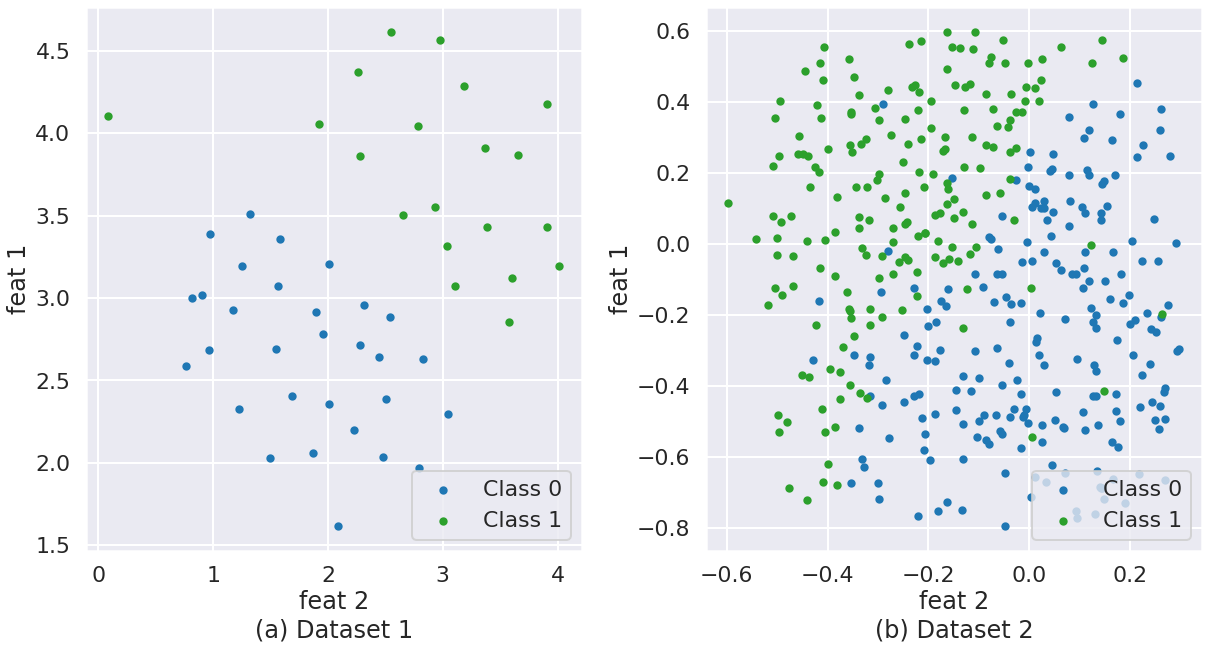
\includegraphics[width=\linewidth]{Img/Q1/Q1_1_Datasets.png}
    \caption{Scatterplots for Dataset 1 (a) and Dataset 2 (b).}
    \label{fig:Q1_1_Datasets}
\end{figure}

\subsection{Question 2: SVM training using different C values}
\label{subsec:Q1_2}
With the two datasets described in \ref{sec:Q1} and plotted in \ref{subsec:Q1_1}, multiple SVMs were trained using different values for the C parameter. The values used for the training were $0.001$, $0.001$, $0.1$, and $1$, for a total of 8 SVMs trained between both datasets. 

\subsection{Question 3: Decision boundary plotting}
\label{subsec:Q1_3}
In addition to the SVMs trained in \ref{subsec:Q1_2}, SVMs with a C value of $10$ and $100$ were also trained to further increase the comaprison pool.  The decision boundary for each of the SVMs trained in \ref{subsec:Q1_2}, with the addition of also training SVMs with a  plotted in combination with the scatterplot of the dataset used to train the respective SVMs. Fig. \ref{fig:Q1_3_SVM1} and Fig. \ref{fig:Q1_3_SVM2} displays the decision boundaries found for Dataset 1 and Dataset 2, respectively.

\begin{figure}[tb]
    \centering
    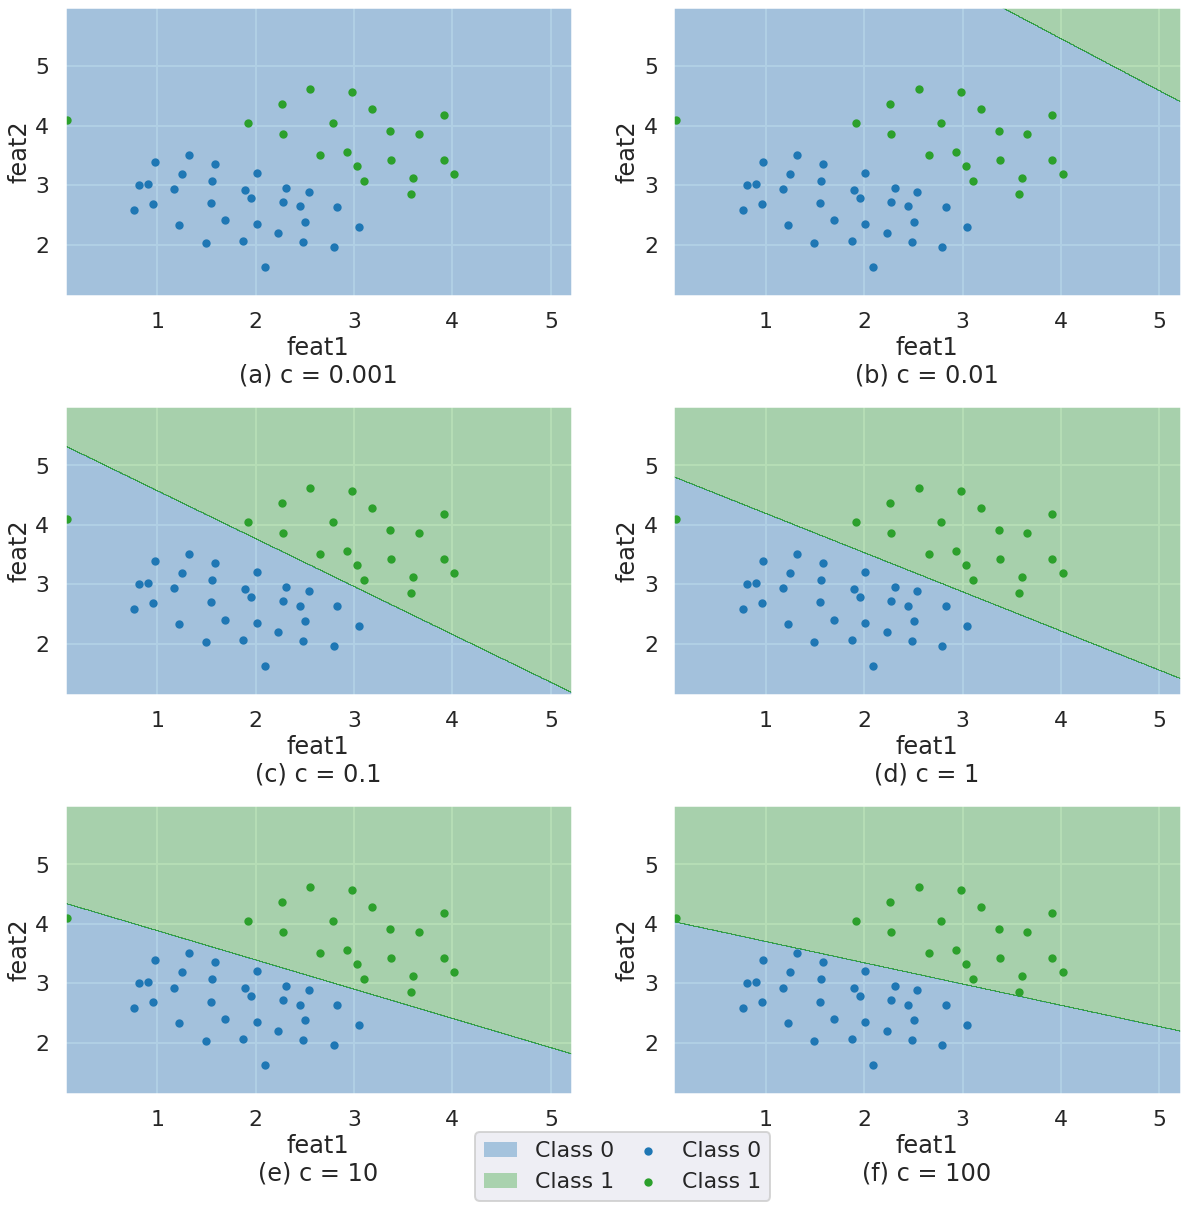
\includegraphics[width=\linewidth]{Img/Q1/Q1_3_SVM1.png}
    \caption{Scatterplot and decision boundaries for SVMs with different values of C on Dataset 1.}
    \label{fig:Q1_3_SVM1}
\end{figure}

\begin{figure}[tb]
    \centering
    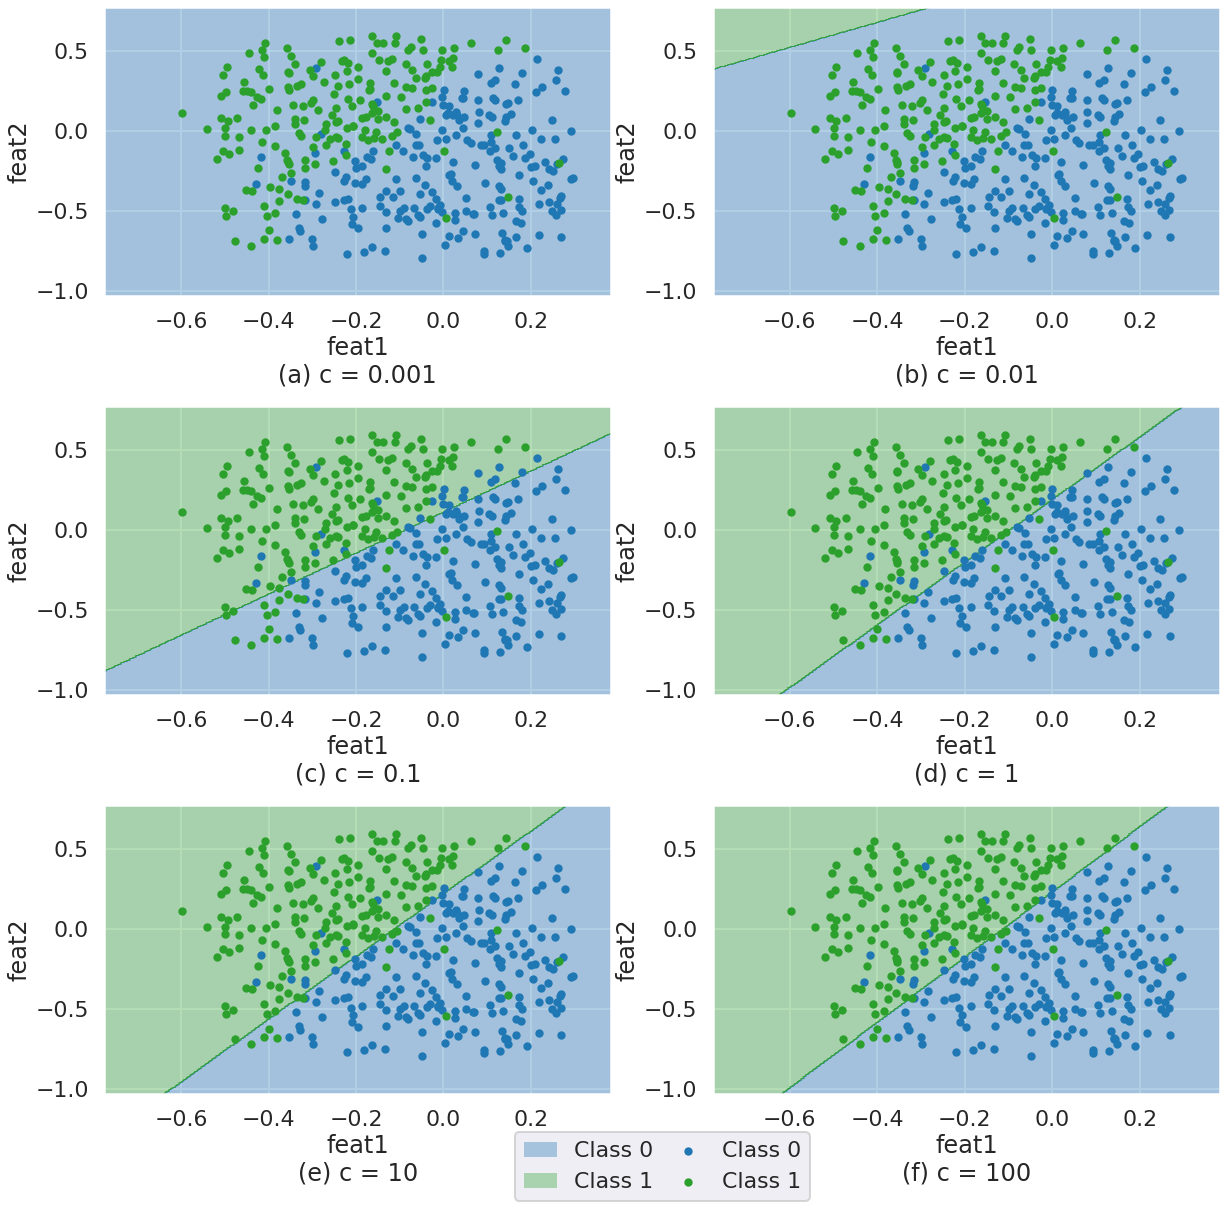
\includegraphics[width=\linewidth]{Img/Q1/Q1_3_SVM2.png}
    \caption{Scatterplot and decision boundaries for SVMs with different values of C on Dataset 2.}
    \label{fig:Q1_3_SVM2}
\end{figure}

In both datasets, it can be seen that with a C value of $0.001$ or $0.01$, the SVM is not able of distinguishing correctly between classes. However, from $C=0.1$ onwards the SVMs are able of classifying values each with a different margin between the support vectors. This difference will be analyzed in further detail in \ref{subsec:Q1_4}.

\subsection{Question 4: Decision boundary plotting}
\label{subsec:Q1_4}
The C value is the parameter that...



Comparing the different C values for the SVMs trained on Dataset 1, it can be argued that the best parameter would be with a C value of $100$, as this value allows for the classification of all the datasamples in their corresponding class. However, this might not be appropriate as the resulting margin is considerably small. What this means is that it might be easy for the SVM to missclassify samples that are close to the decision boundary. Additionally, it is uncertain if the datasample that is close to the coordinates $(0,4)$ is in reality a sample or an outlier as it is the only sample that is not close to the rest of the values for its class. What this implies is that the SVM with a C value of $100$ would have been optimized to contain an outlier and thus it would reduce the final accuracy of the system. With this in mind, a better classifier might be one with a C value between $0.1$ and $10$. The plots for $C=0.1$ and $C=10$, although displaying a correct decision boundary, tend to have a smaller margin than the one for $C=1$, while still retaining the problem of missclassifying the sample in the coordinates $(0,4)$. Assuming that coordinate as an outlier as before, the best classifier would then be the one with the largest margin between both classes, which would mean it would be the classifier with $C=1$.

For Dataset 2, even though $C=0.1$ does classify some values into their respective class, it seems to have a larger missclassification than the SVMs trained with a larger C. At the same time, with this dataset it is not possible to create a margin that correctly separates both classes like in Dataset 1, as there are samples from one class intertwined in what could be considered the opposite's data space. Additionally, the possible margin that can be created between the different classes is narrower than that of Dataset 1, as the classes are closer in space than those of Dataset 1. Taking all of this into account, the SVM with $C=10$ seems to be the one that has a lesser amount of missclassificationsi n the decision boundary, and thus could be argued that is the most suitable.

\section{Question 2: Adaboost}
\label{sec:Q2}
This question involved creating linear SVMs to classify data from a dataset with two classes. Apart from this, the Adaboost Ensemble technique was used to create a classifier combining the technique with SVM classifiers.
% -----------------------b--------------------------------------------------
\bibliographystyle{IEEEbib}
\bibliography{strings,refs}

\end{document}
